\section{Anhang}
	\subsection{Abbildungen}
	\begin{figure}[!ht]
		\centering									% Bild Zentrierung
		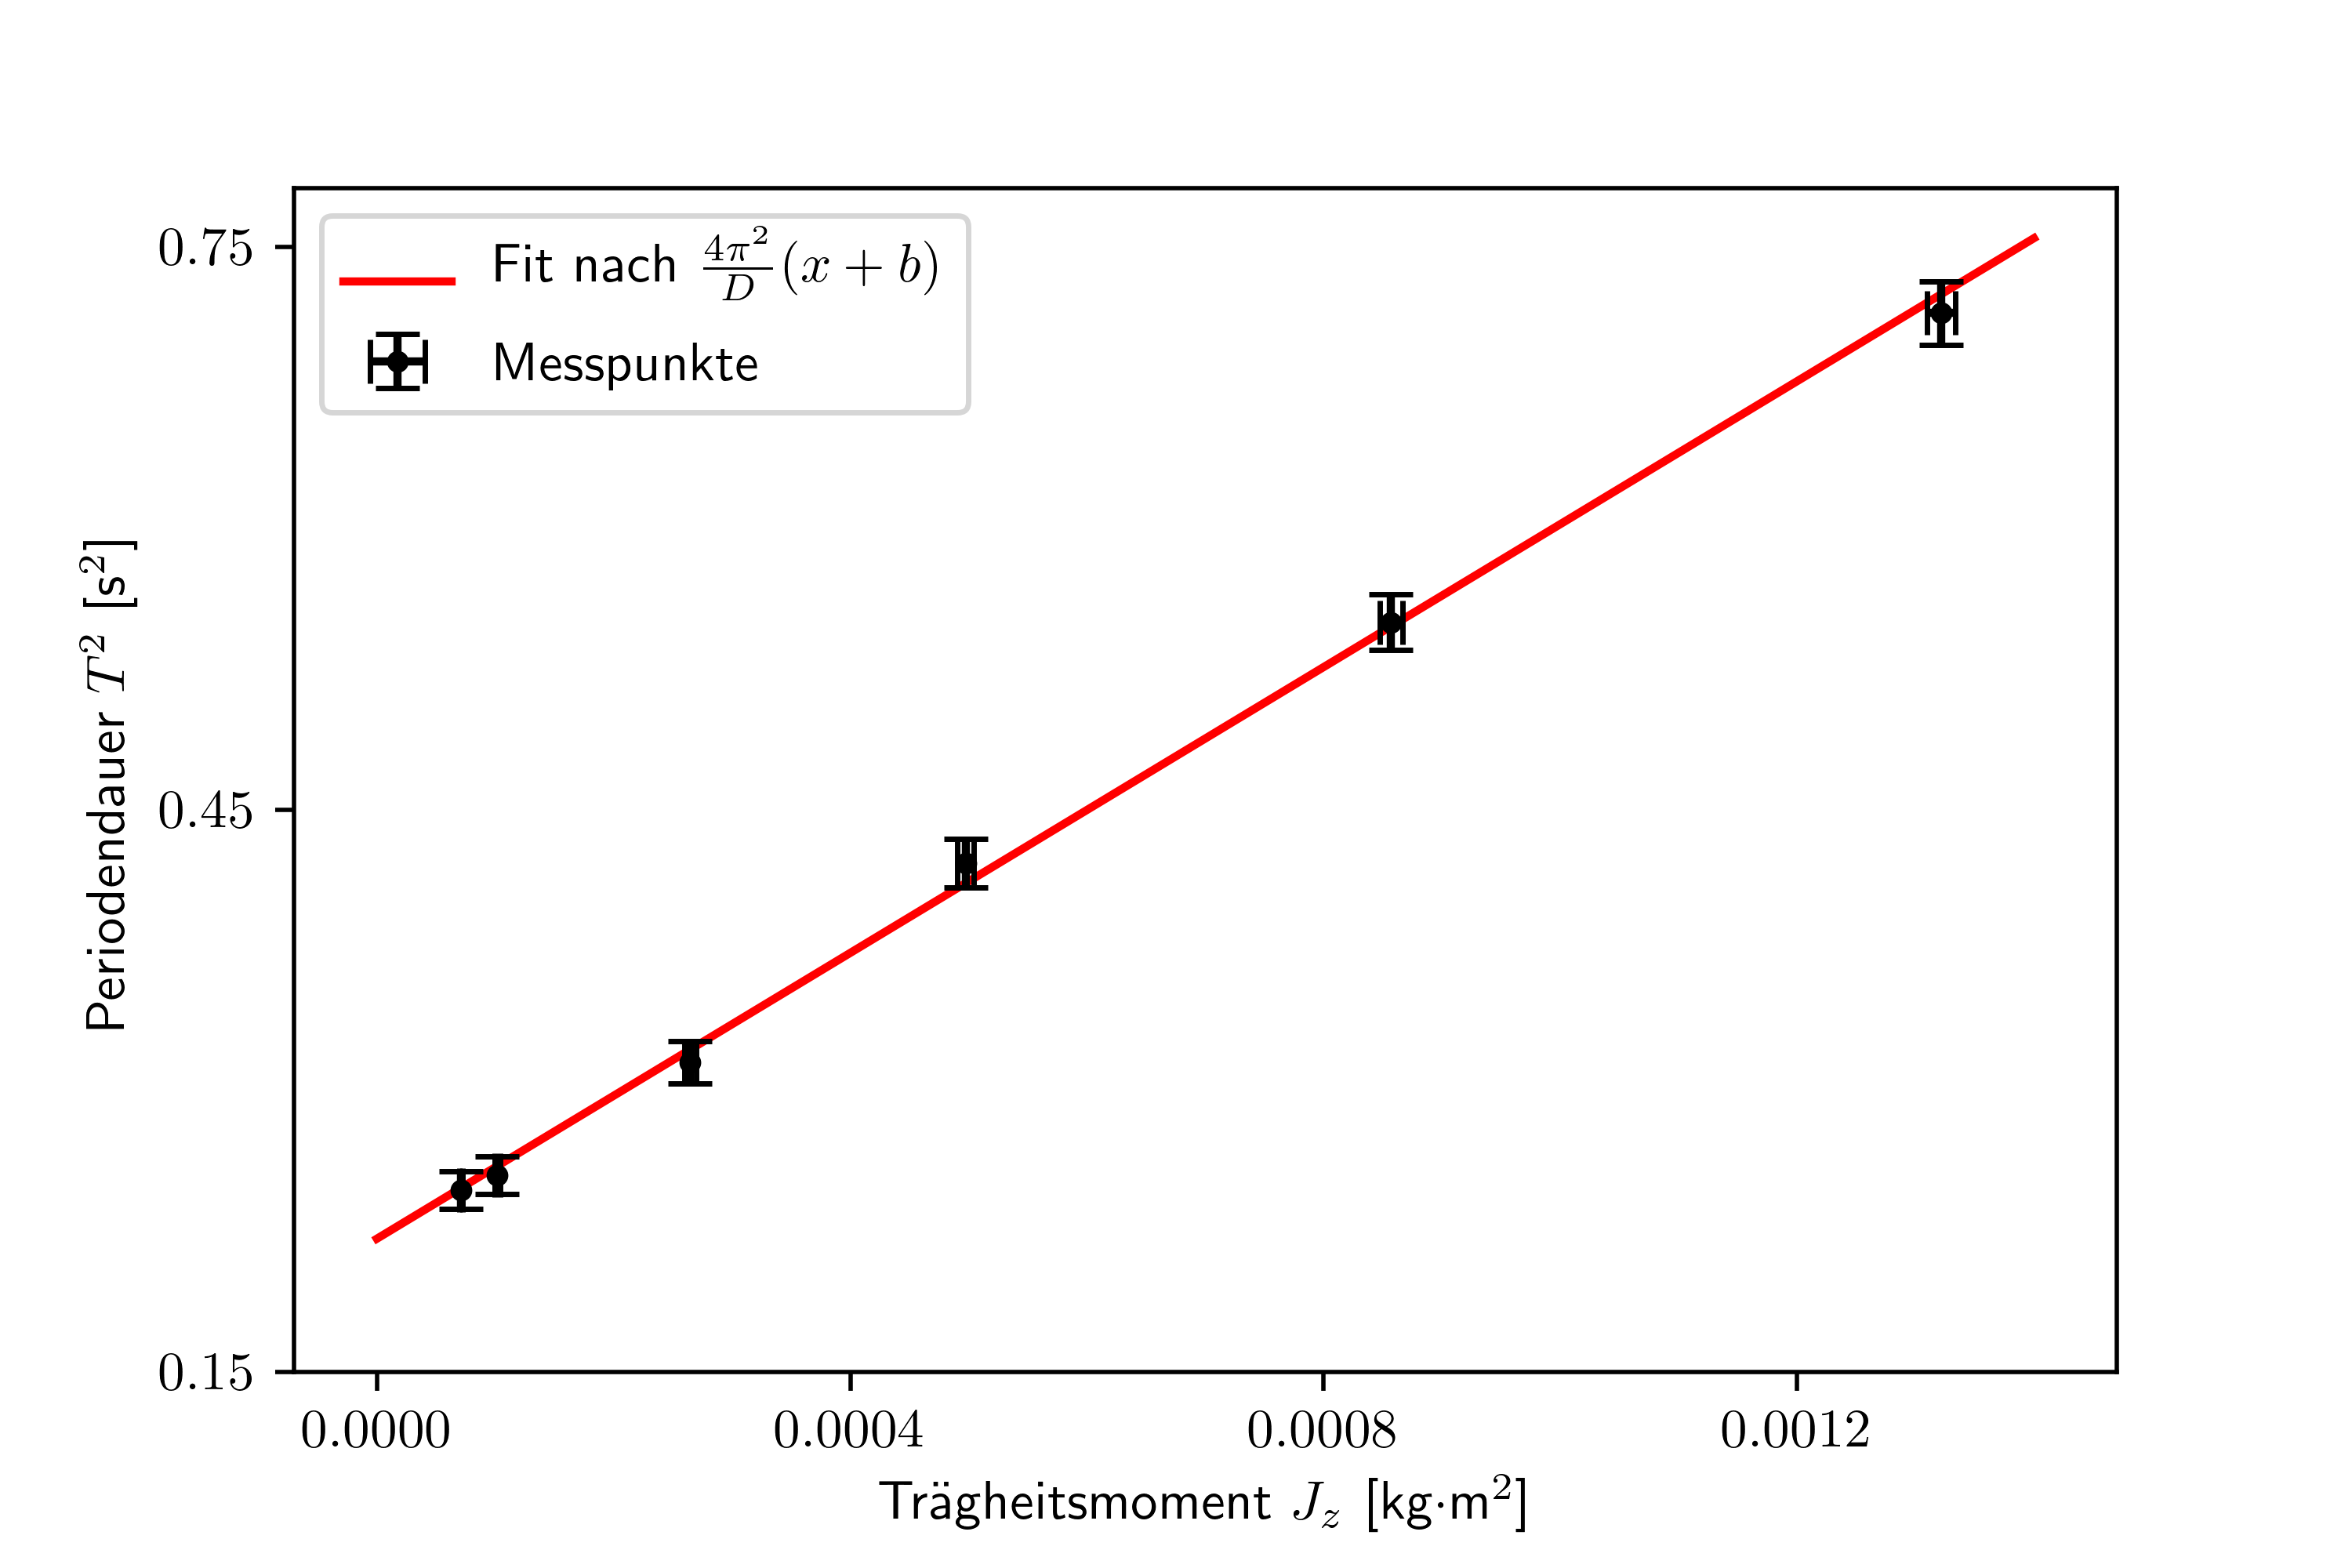
\includegraphics[width=300pt]{fotos/gpr1/Regression_M2_J_Tisch.png}			% einfügen des Bildes/ mit width Bildbreite einstellen
		\caption{Linearität zwischen quadrierter Periodendauer $ T^{2} $ und Trägheitsmoment $ J_{Z} $. Fehlerbalken sind durch Fehlerfortpflanzung entstanden. Abbildung zeigt gemittelte Werte für $ T^{2} $ aus der Tabelle (\ref{Tab: J_Tisch}). $ R^{2}=0.999 $. $ \chi^{2}=2.50 $ }							% Bildunterschrift
		\label{Abb.: J_Z}							% für Textverweise
	\end{figure}

\begin{figure}[!ht]
	\centering									% Bild Zentrierung
	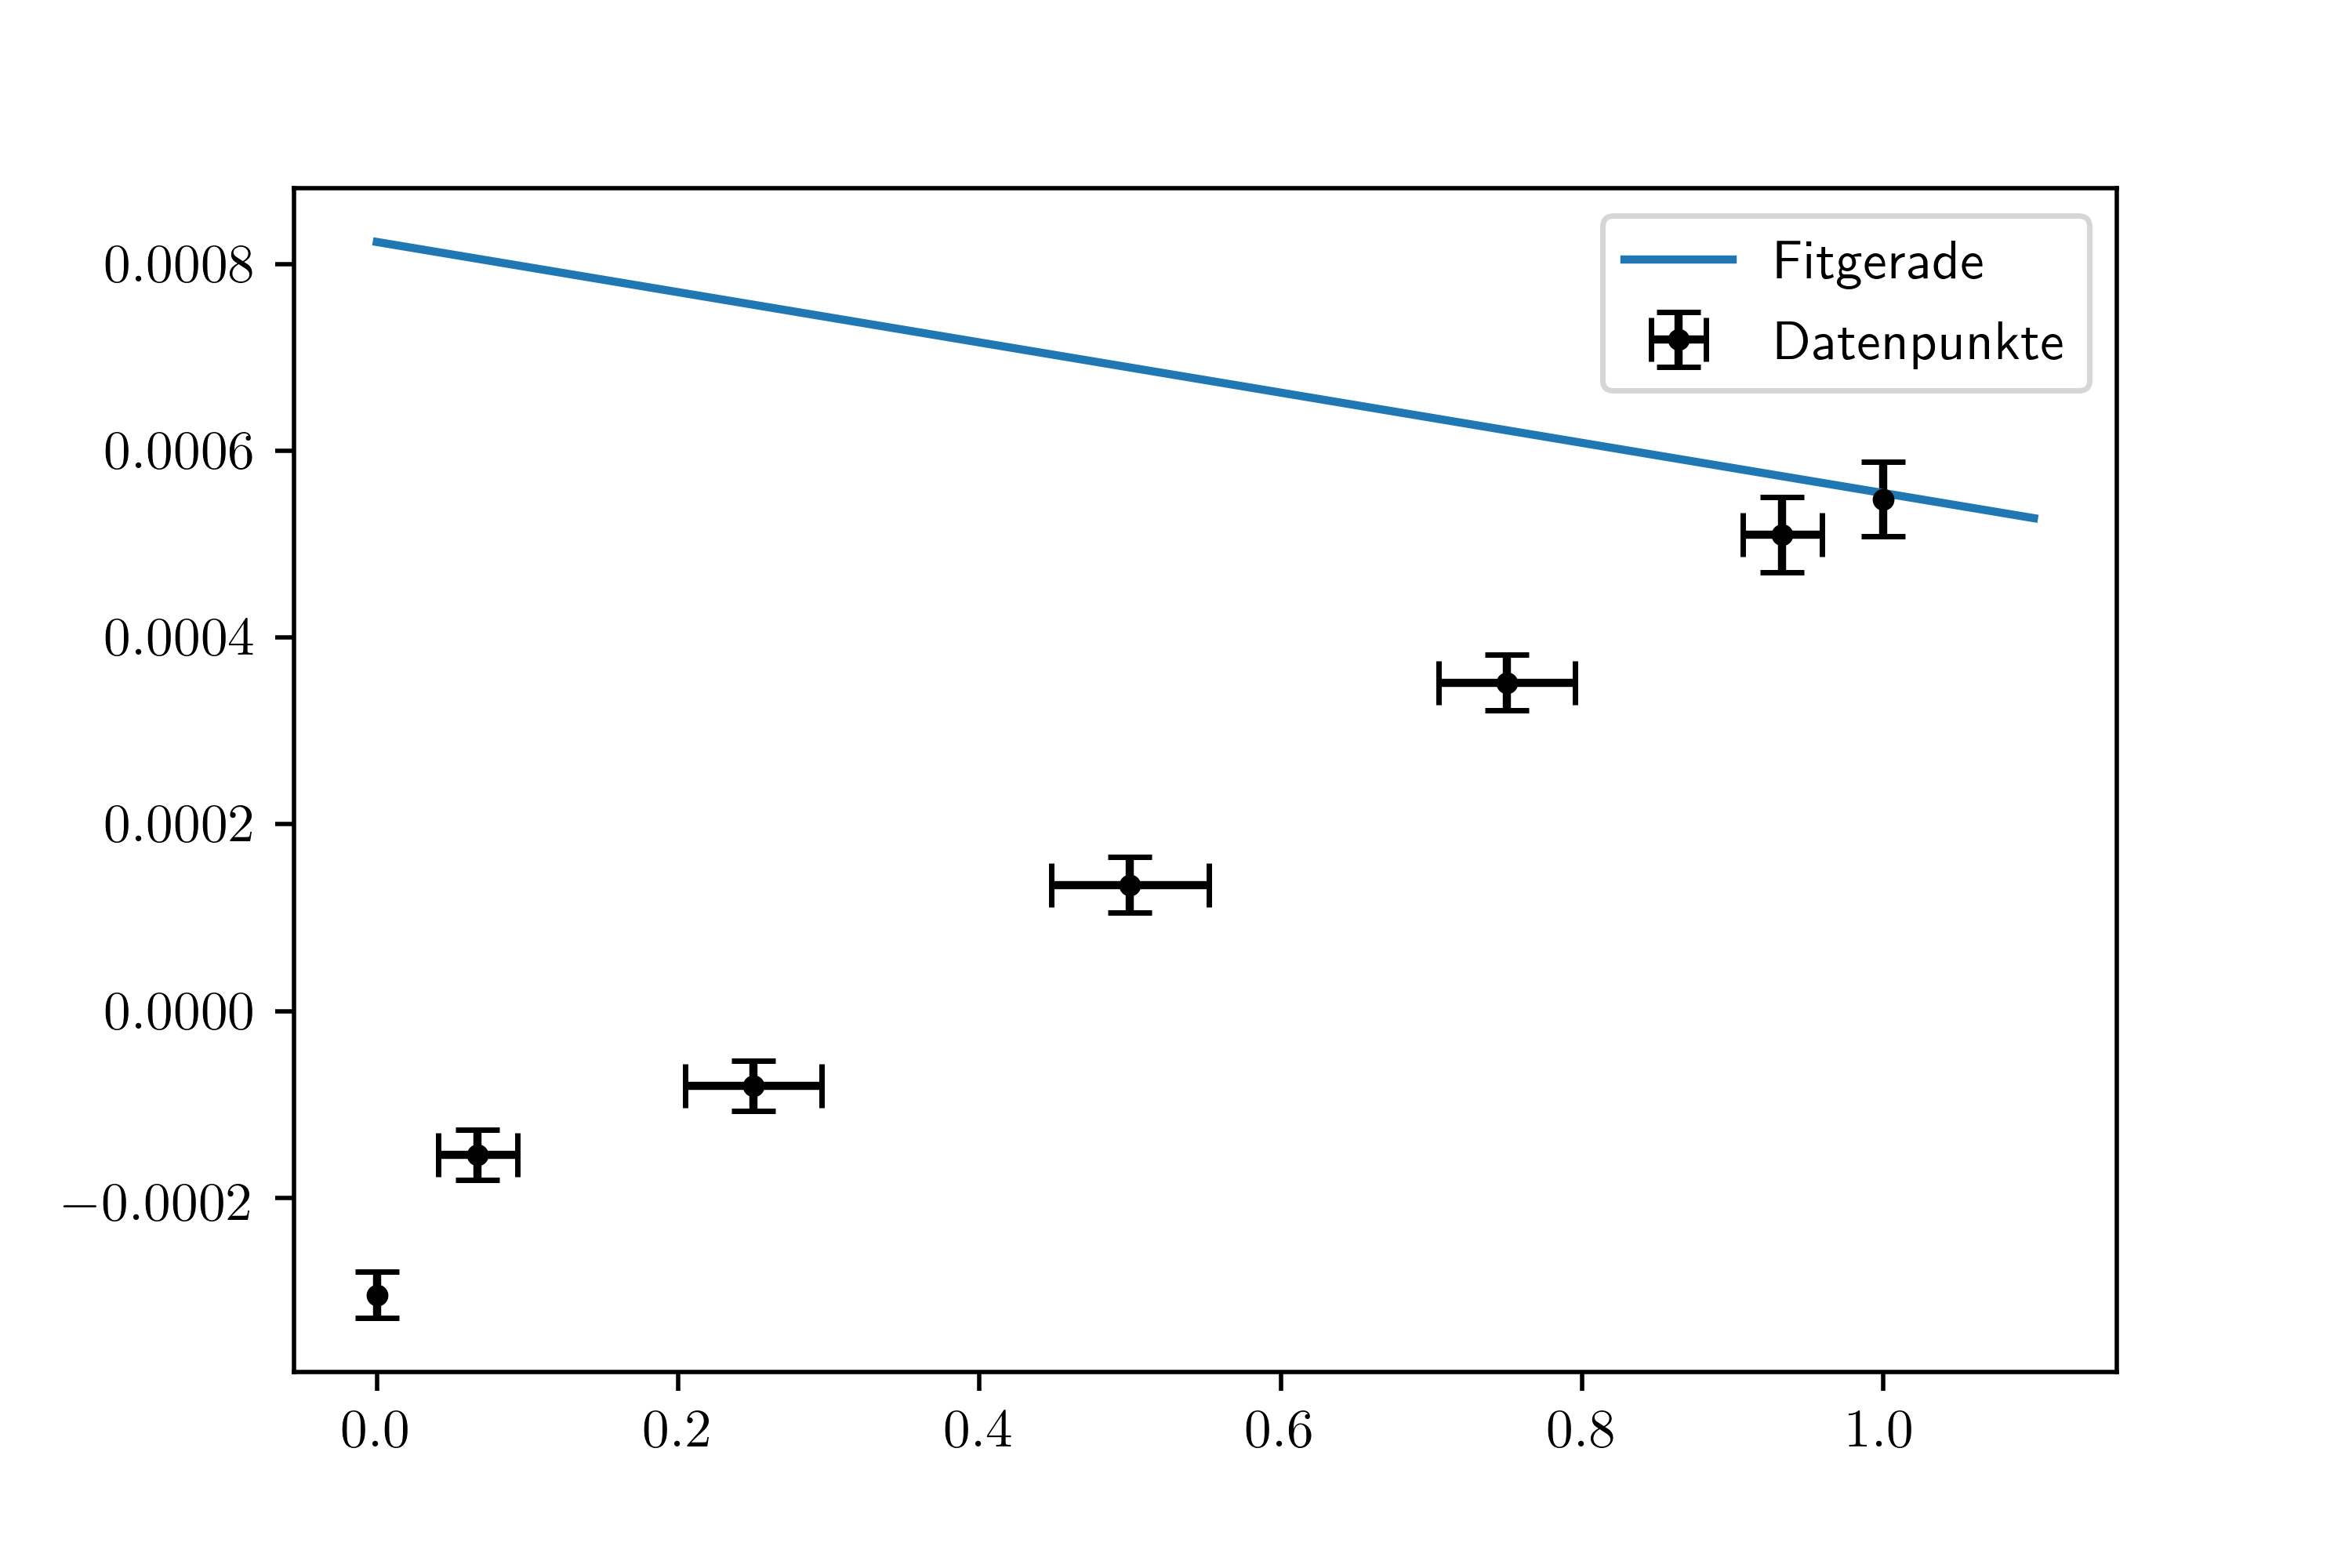
\includegraphics[width=300pt]{fotos/gpr1/Regression_Zylinder.png}			% einfügen des Bildes/ mit width Bildbreite einstellen
	\caption{Linearität zwischen $ J_{\gamma} $ und $ \sin^{2}(\gamma) $. Abbildung zeigt gemittelte Werte von $ T^{2} $ aus der Tabelle (\ref{Tab: sin}). $ R^{2}=0.992 $, $ \chi^{2}=6164.4 $ }							% Bildunterschrift
	\label{Abb.: gam}							% für Textverweise
\end{figure}
	